In this section, we shall describe a model for simulating the chipping of a stone. In particular, we think of the erosion of a stone as coming from shear forces. This discrete model for eroding the stone allows us to simulate random processes and view the shape of a stone after some number of time steps. We provide computer simulations for the erosion process and analyze the model through these simulations.

\subsection{Shearing Stones}

The discrete model for stone erosion is based on the idea that stones are eroded via chipping. The process of chipping is analogous to dropping a stone from a specified height and applying a shear force to a particular point on the stone. Intuitively, one can think of a stone in a stream being eroded by being tossed and turned by the force of the river. This tossing and turning causes the stone to collide with other stones on the bottom of the riverbed, causing chipping to occur.

We model the interaction between two stones as a shear force, a force that causes two parts of a stone to move in opposite directions. The point where a stone collides with another stone is the point where the shear force is concentrated. This causes the stone to break into two pieces. The processes by which shear forces cause breakages in materials are extremely complicated, so we will use the following simple assumption: we shall assume that the amount of volume that is sheared off of a stone is proportional to the amount of force incident on the stone.

\subsection{Definitions}

This section will define how we represent a stone in the discrete model. We will represent a stone as a polygon in $k$-dimensional space with $n$ vertices.

\begin{definition}
  A polygon $s$ consisting of $n$ vertices is defined by the set of vertices $s = \{ \bvec{v}_0, \ldots, \bvec{v}_{n-1} \}$ where each vertex $\bvec{v}_i \in \mathrm{R}^k$ is a tuple. Vertices $\bvec{v}_i$ and $\bvec{v}_{i+1}$ are connected by a line segment for all $i \in \{0, 1, \ldots, n \}$ and the line segments do not intersect each other, except at the vertices.
\end{definition}

When referring to vertices, we will use the convention of taking vertex indices modulo $n$ for convenience. Hence $v_{i \mod{n}} \equiv v_i$. Note that this means that $v_{n} = v_{0}$ so that vertex $v_{n-1}$ has a line segment connecting it to $v_{0}$.

The centroid $\bvec{c}_s$ of a stone $s$ is the center of mass of the stone when the stone has uniform density. In other words, the centroid is the point $\bvec{c}_s \in \mathrm{R}^k$ where the following holds:

\begin{eqnarray}
 \int_V (\bvec{r} - \bvec{c}_s) dV = 0
\end{eqnarray}

Where $V$ is the area of the stone, using all values $\bvec{r} \in V$. 

In addition, we will define a pseudo-probability distribution, which we will use to generate random points on a line.

\begin{definition}
  A pseudo-probability distribution $\mathrm{P}(x, y)$ defines $Pr[i | \mathrm{P}]$, the probability of selecting some $i \in \mathrm{R}$, such that $Pr[i | \mathrm{P}] = 0$ for $i \notin [x,y]$ and $\int_{x}^y Pr[i | \mathrm{P}] di = 1$. We use the notation $j \sim \mathrm{P}(x,y)$ to denote that $j \in [x,y]$ is a realization of a draw from the pseudo-probability distribution $\mathrm{P}(x,y)$. In other words, we select $j$ with probability $Pr[j | \mathrm{P}]$.
\end{definition}

For example, one possible pseudo-probability distribution $\mathrm{P}(x,y)$ would have $Pr[i | \mathrm{P}] = \frac{1}{y-x}$ for all $i \in [x,y]$. This would be the uniform pseudo-probability distribution on a range $[x,y]$.

We will also introduce the notion of a convex vertex, which will be useful when defining our chipping process.

\begin{definition}
  A convex vertex $\bvec{v}_c$ on a polygon $s$ consisting of $n$ vertices is a vertex $\bvec{v}_i$ which, when removed from the polygon $s$ to create a new polygon $s' = \{ \bvec{v}_0, \ldots, bvec{v}_{i-1}, \bvec{v}_{i+1}, \ldots, \bvec{v}_{n-1} \}$ has the property $V(s) \geq V(s')$ (where $V(\cdot)$ denotes the volume of a stone).
\end{definition}

In the following sections, we will assume that one cannot chip a vertex which is not convex. The reasoning relies on our intuition for how a stone chips. Non-convex vertices can be thought of as moving in towards the center of a stone, and chipping a stone can be thought of being caused by the stone crashing into the ground. It is impossible for a stone to be chipped on a vertex which is not convex if the stone is falling onto a flat surface (the protruding vertices surrounding the convex vertex will be chipped first). Therefore, we make the assumption that convex vertices are the only ones which can be chipped through our mechanism.

\subsection{The Chipping Process Model}

With this in mind, we shall now develop a model for the chipping of a stone based on shearing. We will confine our work to $\mathrm{R}^2$. The main idea of the model is that we will represent a stone as a two-dimensional polygon, and chip off a constant amount of area of the stone at every time step. In this way, we will attempt to capture the process of a stone colliding with another stone on a riverbed. Randomness will be introduced into the model by randomly selecting somewhere on the stone to start the shearing.

We shall now give a formal definition of the chipping process. A chip for a pseudo-probability distribution $\mathrm{P}(0,1)$, stone $s$, and area $A$ is denoted $Chip(\mathrm{P}, A, s)$ and is represented as follows:

\begin{enumerate}
  \item Select a vertex $\bvec{v}_j$ from $s$. To select this vertex, we find the centroid $\bvec{c}_s$ of stone $s$ and choose an angle $\gamma \in [0, 2\pi)$ uniformly at random. Now, define the ray $\bvec{l}$ as the ray with an initial point of $\bvec{c}_s$ which extends outwards infinitely at an angle of $\gamma$ from the horizontal. The vertex with the minimum perpendicular distance to $\bvec{l}$ will be $\bvec{v}_j$. Repeat this process as many times as necessary until we have selected a convex vertex.
  \item Given vertex $\bvec{v}_j$, define $\bvec{l}_l$ as the line segment which connects $\bvec{v}_j$ and $\bvec{v}_{{j-1}}$. Similarly, define $\bvec{l}_r$ as the line segment connecting $\bvec{v}_j$ and $\bvec{v}_{{j+1}}$ (recall that our convention is to take the vertex indices modulo $n$).
  \item Select $\bvec{l}_1$ from the set $\{ \bvec{l}_l, \bvec{l}_r \}$ uniformly at random (i.e. $Pr[\bvec{l}_1 = \bvec{l}_l] = Pr[\bvec{l}_1 = \bvec{l}_r]$). Call the line segment which was not selected $\bvec{l}_2$.
  \item Select a point $\bvec{p}_1$ at random from $\bvec{l}_1$. To do this, we select a random $t \sim \mathrm{P}(0,1)$ and let $\bvec{p}_1 = \bvec{v}_j t + (1-t) \bvec{v}_{{j-1}}$. Recall that $t \sim \mathrm{P}(0,1)$ denotes that $t$ is drawn from the pseduo-probability distribution $\mathrm{P}(0,1)$.
  \item Select the point $\bvec{p}_2$ which lies on $\bvec{l}_2$ for which the polygon defined by $\{\bvec{p}_1, \bvec{v}_j, \bvec{p}_2\}$ has an area of $A$. If no such polygon exists, then choose $\bvec{p}_2 = \bvec{v}_{{j+1}}$.
  \item Create a new stone $s'$ whose vertices are given by
    \begin{eqnarray*}
      s' = \{ \bvec{v}_1, \ldots, \bvec{v}_{j-1}, \bvec{p}_1, \bvec{p}_2, \bvec{v}_{j+1}, \ldots, \bvec{v}_n \}
    \end{eqnarray*}
    Here, the vertex $\bvec{v}_j$ has been replaced by $\bvec{p}_1$ and $\bvec{p}_2$ in the list of vertices for $s$. The new stone $s'$ now has one more line segment and vertex than the old stone $s$.
\end{enumerate}

Now that we have defined a chip $Chip(\mathrm{P}, A, s)$, we can define our entire model as a chipping process.

\begin{definition}
A chipping process for a probability distribution $\mathrm{P}$, stone $s$, area $A$, and iterations $k$ is denoted $ChipProcess(\mathrm{P}, A, s, k)$. A chipping process returns a stone $s'$ which has iteratively conducted $k$ chips. Thus, a chipping process takes a stone $s$ and creates $s_1 = Chip(\mathrm{P}, A, s)$, $s_2 = Chip(\mathrm{P}, A, s_1)$, \ldots, $s_k = Chip(\mathrm{P}, A, s_{k-1})$, and returns $s' = s_k$.
\end{definition}

\subsection{Simulations}

The chipping process model allows us to simulate changes to a stone. A stone which undergoes a chipping process should have a shape which is close to the stones which undergo erosion and chipping in the real world (if our chipping process model is an accurate description of erosion).

To examine the accuracy of our model, we performed computer simulations using the Python programming language and the Shapely library. With computer simulations, we were able to create multiple instances of a chipping process and analyze the shapes of the resulting stones. We were also able to use multiple probability distributions $\mathrm{P}$ and areas $A$ to generate different chipping processes.

\begin{figure}
  \begin{center}
    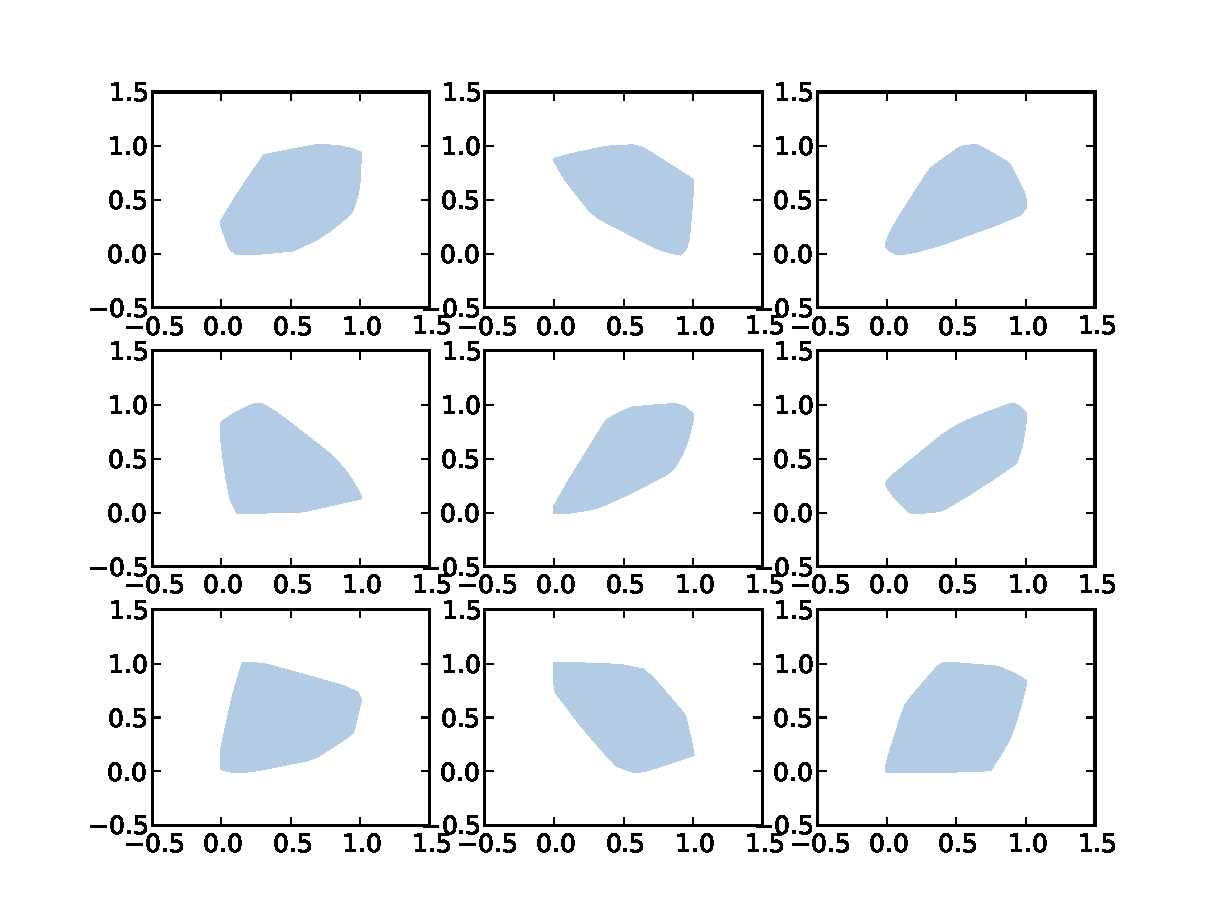
\includegraphics[width=4in]{area_chipper_sample.pdf}
  \end{center}
  \caption{Chipping Process for a Unit Square \label{fig:area_chipper_sample}}
\end{figure}


For our simulations, we use a pseudo-probability distribution $\mathrm{P}(0,1)$ which is a normal distribution with mean $\mu$ and standard deviation $\sigma$. We select $\mu \in [0,1]$ and all realizations of the normal distribution which fall outside of $[0,1]$ are discarded and we select a new element from the normal distribution. We will denote a pseudo-probability distribution which is using a normal distribution with $\mathrm{P}(0,1) = \mathrm{N}(\mu, \sigma)$.

Figure \ref{fig:area_chipper_sample} shows the results for nine chipping process runs. The parameters used in these runs were $\mathrm{P} = \mathrm{N}(0.5, 0.15)$, $A = 0.05$, $k = 50$, and $s = \{(0,0), (1,0), (1,1), (0,1)\}$. The chipping processes each started out with a stone which was a unit square. The stones were chipped 50 times by the method described by the model. The probability distribution $\mathrm{P}$ is a normal distribution so that $t = 0.5$ is the most likely $t$ to choose. In other words, it is most likely that $\bvec{p}_1$ will be chosen as the midpoint of the line segment $\bvec{l}_1$.

This distribution was chosen because it is more likely that shear forces will cause a symmetric split about the vertex $\bvec{v}_j$. However, it is still possible for non-symmetric splits to occur, i.e. when $t \neq 0.5$. The normal distribution captures this nicely (all realizations of $t$ which are not in the interval $[0,1]$ were discarded).

Figure \ref{fig:area_chipper_sample} displays the typical results of the chipping process model. None of the stones resemble a square and it would be hard for anyone to have guessed that these shapes came from a common origin. In fact, the randomization from the distribution $\mathrm{P}$ makes all of the shapes slightly different.

To examine the chipping process more closely, we can look at how circular or elliptical the resulting shapes are. One would expect rocks in a stream or riverbed to be elliptical in shape. We can therefore examine the distance of random points on a stone from the centroid. We will generate a large number of random points, and plot their distances from the centroid.

More precisely, a random point $\bvec{p}_s$ on the stone $s$ will be selected by the following process:
\begin{enumerate}
  \item Produce a random angle $\theta \in [0, 2\pi)$, drawn uniformly from the range $[0, 2\pi)$.
  \item Draw a ray from the centroid of the stone with an angle $\theta$ from the horizontal (x-axis).
  \item The ray will intersect with the stone in exactly one location (since the stone is closed). Set the random point $\bvec{p}_s$ as the point where the ray intersects an edge on the stone.
\end{enumerate}

When we plot the distances, we will scale the distances to the centroid of a point $\bvec{p}_s$, denoted by $d(\bvec{p}_s, \bvec{c}_s)$. We will sample $q$ random points from the stone, and plot the scaled distances. Let $\min_d = \min d(\bvec{p}_s, \bvec{c}_s)$ be the minimum observed distance and $\max_d = \max d(\bvec{p}_s, \bvec{c}_s)$ be the maximum observed centroid distances for the $q$ samples on a stone $s$. We will define the scaled distance to the centroid of a stone $s$ as $d'_s(\bvec{p}_s, \bvec{c}_s)$ with the following formula:

\begin{eqnarray}
  d'_s(\bvec{p}_s, \bvec{c}_s) = \frac{d(\bvec{p}_s, \bvec{c}_s) - \min_d}{ \max_d - \min_d }
\end{eqnarray}

We can get intuition for this metric by examining common shapes. In a circle, all of the distances to the centroid would be the same. In an elipse, one would expect a skewed curve, with more points lying closer to the centroid. One can see this by examining all points on an ellipse which have distances from the centroid lying in $[d, d + \epsilon]$. The slices of the ellipse which are carved out will have strictly greater total angle than the angles carved from using distances in $[d + \epsilon, d + 2 \epsilon]$.

\begin{figure}
  \begin{center}
    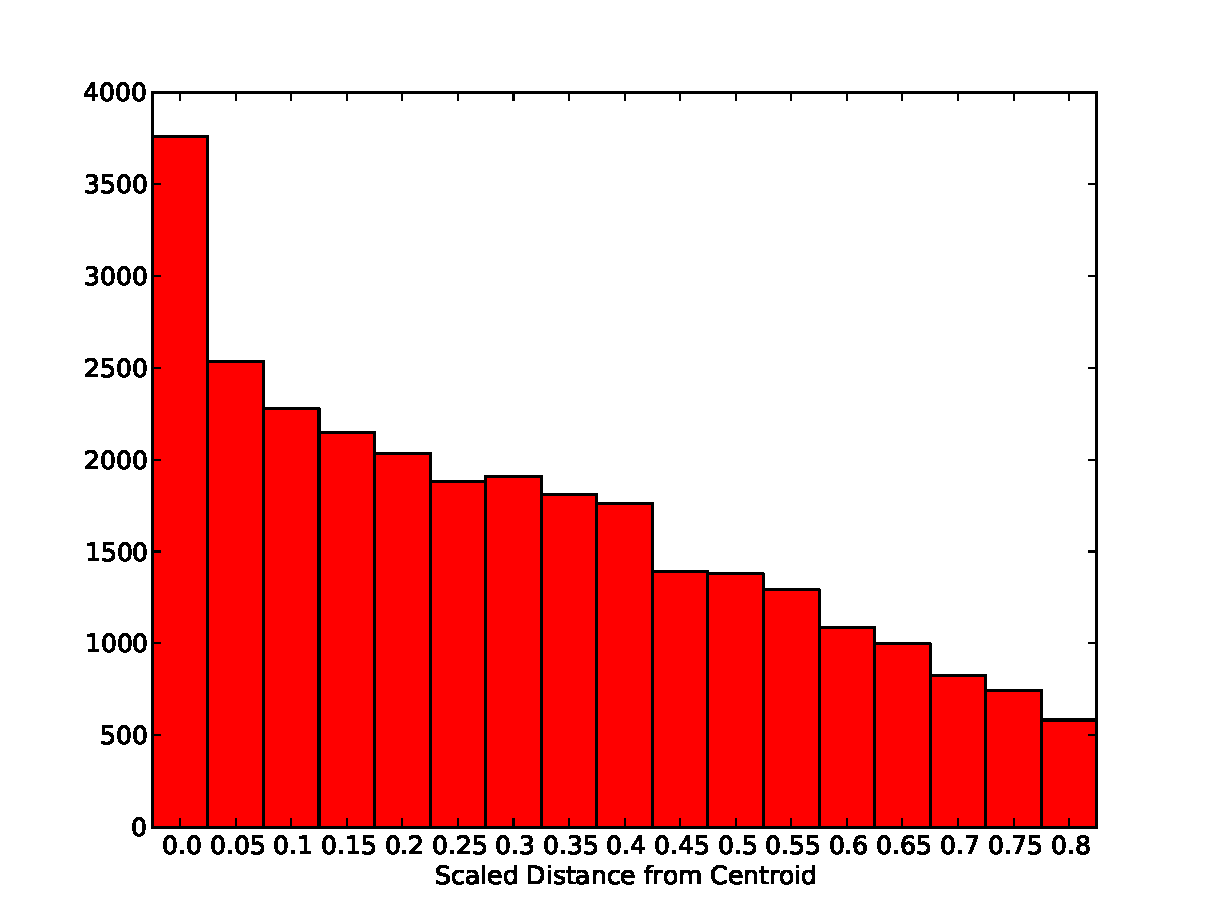
\includegraphics[width=4in]{distance_from_centroid.pdf}
  \end{center}
  \caption{Histogram of Vertex Distance From Centroid \label{fig:distance_from_centroid}}
\end{figure}

Figure \ref{fig:distance_from_centroid} shows the distribution of vertex distances which were simulated with the same parameters as used for figure \ref{fig:area_chipper_sample}. One can see that the distribution is skewed, with most points being closer to the centroid. The distribution of vertex distances from the centroid show that the shapes that result from this set of chipping process conditions have a similar distribution as an ellipse would.
